\documentclass{beamer}
\usetheme{Boadilla}

\title{House sale price predictions}
\subtitle{Using tree-based algorithms and recursive feature elimination (RFE)}
\author{Julian Cabezas Pena}
\institute{a1785086}
\date{\today}

\begin{document}
	
\begin{frame}
	\titlepage
\end{frame}	


\begin{frame}
	\frametitle{Introduction}
	
	\begin{itemize}
		\item Regression problem: Continuous target variable
		\item Bagging and Boosting algorithms: combine various learners (decision trees) to accomplish improved predictions
		\item Kaggle competition to predict house prices using the Ames, Iowa dataset
	\end{itemize}
	
\end{frame}


\begin{frame}
	\frametitle{Tested methods}
	
	\begin{itemize}
		\item Random Forest: Uncorrelated trees in parallel
		\item Gradient Boosting: Trees in sequence
		\item Extreme Gradient Boosting (XGBoost): Popular on competitions
		\item Categorical Boosting (CatBoost): Developed by Yandex, new (2018)
	\end{itemize}
	
\end{frame}


\begin{frame}
	\frametitle{Data preprocessing}
	
	\begin{itemize}
		\item Missing values: Handing according to documentation
		\item Missing values: According to neighbourhood median or mode
		
		\begin{figure}[H]
			\begin{center}
				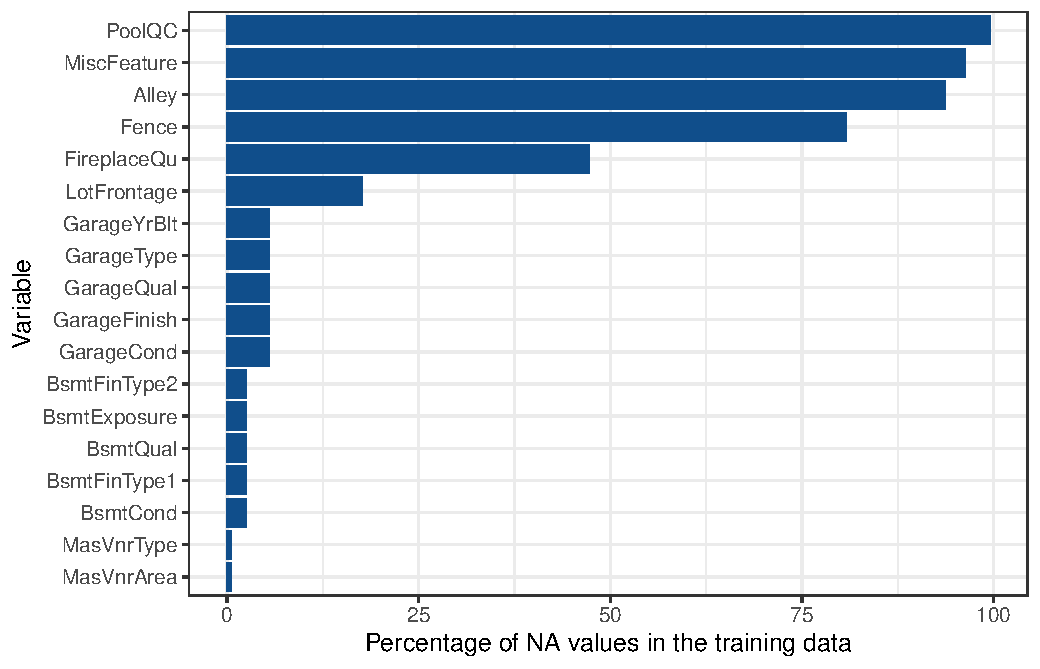
\includegraphics[width=0.8\linewidth]{NA_plot.pdf}
			\end{center}
			\label{fig:log}
		\end{figure}
		
	\end{itemize}
	
\end{frame}

\begin{frame}
	\frametitle{Data preprocessing}
	
	\begin{itemize}
		\item One hot encoding of categorical variables
		\item Log Transformation of target variable
		
		\begin{figure}[H]
			\begin{center}
				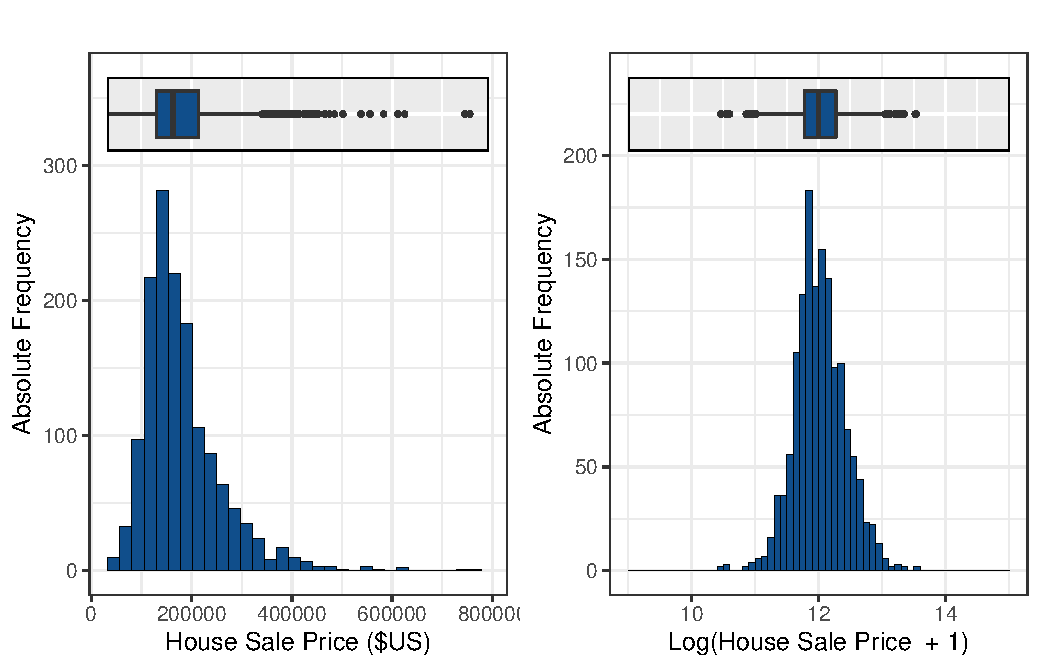
\includegraphics[width=0.8\linewidth]{2hist_saleprice.pdf}
			\end{center}
			\label{fig:log}
		\end{figure}
		
	\end{itemize}
	
\end{frame}


\begin{frame}
	\frametitle{Recursive Feature Elimination}
	
	\begin{itemize}
		\item Allows to drop redundant or unimportant features (5 fold CV)
		
		\begin{figure}[H]
			\begin{center}
				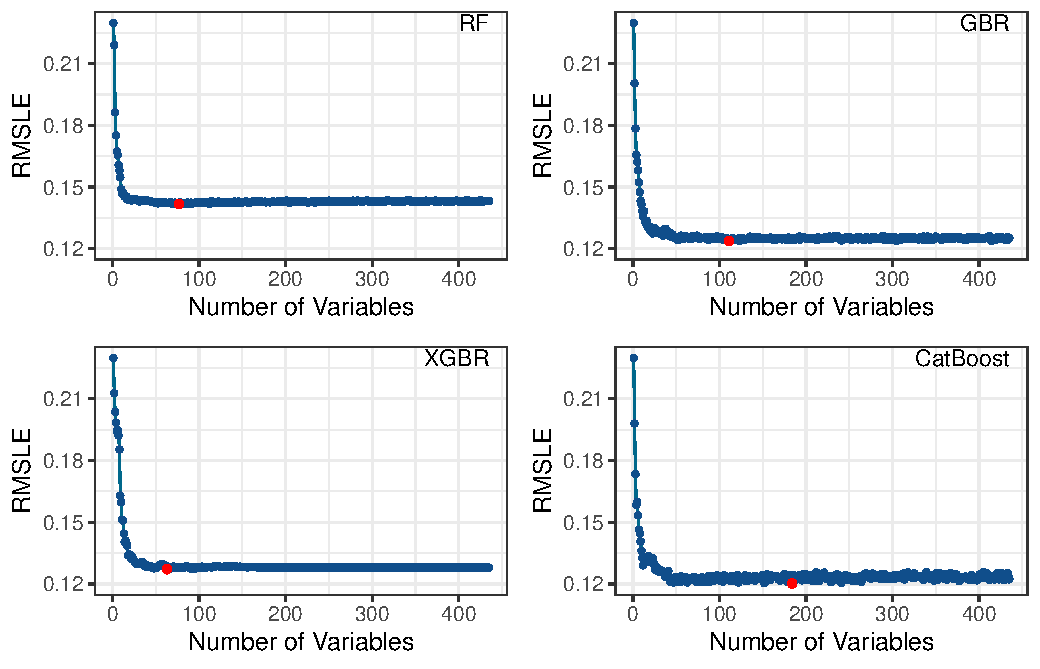
\includegraphics[width=0.8\linewidth]{RFE.pdf}
			\end{center}
			\label{fig:rfe}
		\end{figure}
		
	\end{itemize}
	
\end{frame}

\begin{frame}
	\frametitle{Parameter Tuning}
	
	5-fold cross validation, 3 sets of 3 parameters tested
	
\begin{table}[H]
	\begin{center}
		\begin{tabular}{|p{1.5cm}|p{7cm}|p{2cm}|}
			\hline
			Algorithm & Tuned parameters & RMSLE (CV) \\
			\hline\hline
			RF & $n_\mathrm{trees} = 1500$, $max_\mathrm{features} = 22$ \&  $max_\mathrm{depth} = none$ & 0.1356\\
			GB & $n_\mathrm{trees} = 1000$, $learning rate = 0.1$ \& $depth = 4$ & 0.1184\\
			XGBoost  & $n_\mathrm{trees} = 500$, $learning rate = 0.05$ \& $max_\mathrm{depth} = 3$ & 0.1242 \\
			CatBoost & $n_\mathrm{trees} = 2000$, $learning rate = 0.1$ \& $max_\mathrm{depth} = 6$ & 0.1189\\
			\hline
		\end{tabular}
	\end{center}
	\label{table:tuningres}
\end{table}
	
\end{frame}

\begin{frame}
	
	\frametitle{Testing}
	
	\begin{table}[H]
		\begin{center}
			\begin{tabular}{|p{4.5cm}|p{3cm}|p{3cm}|}
				\hline
				Algorithm & RMSLE (Test set) \\
				\hline\hline
				Random forest & 0.1389 \\
				Gradient Boosting & 0.1372  \\
				Extreme Gradient Boosting  & 0.1369
				\\
				Categorical Boosting & 0.1269\\
				\hline
			\end{tabular}
		\end{center}
		\label{table:test}
	\end{table}

	\begin{figure}
		\centering
		
\includegraphics[width=1.05\linewidth]{screenshot001}
		\label{fig:screenshot001}
	\end{figure}

	Kaggle user: JulianCabezas

\end{frame}


\begin{frame}
	
	\frametitle{Conclusion}
	
	\begin{itemize}
		\item The RFE-Gridsearch workflow, although time consuming, provided good results.
		\item The new CatBoost algorithm looks promising and can be fine-tuned to obtain even better results
	\end{itemize}
	
	
\end{frame}


\end{document}